\documentclass[11pt]{article}

% ---------- packages ----------
\usepackage[a4paper,margin=2.1cm,top=2.6cm,bottom=2.6cm,headheight=24pt]{geometry}
\usepackage[table]{xcolor}
\usepackage{amsmath}
\usepackage{amssymb}
\usepackage{booktabs}
\usepackage{colortbl}
\usepackage{array}
\usepackage{tabularx}
\usepackage{enumitem}
\usepackage{tikz}
\usetikzlibrary{positioning,calc,shapes.geometric,decorations.pathmorphing,backgrounds,patterns}
\usepackage[most]{tcolorbox}
\usepackage{fancyhdr}
\usepackage{fontawesome5}
\usepackage{titlesec}
\usepackage{ragged2e}
\usepackage{pgffor}
\usepackage{blkarray}
\usepackage{lastpage}

% ---------- palette ----------
\definecolor{primary}{HTML}{1B2A4A}   % deep navy
\definecolor{gold}{HTML}{B8892F}      % warm gold accent
\definecolor{slate}{HTML}{5B6472}     % muted slate text
\definecolor{mint}{HTML}{1E7B5C}      % solution-key green
\definecolor{paper}{HTML}{FAF9F6}     % warm off-white
\definecolor{rulegray}{HTML}{D8D3C8}

% ---------- mode switch ----------
% Set \showsolutionstrue for the instructor Solution Key, \showsolutionsfalse
% for the blank Student Copy. Everything below reflows automatically.
\newif\ifshowsolutions
\showsolutionstrue

\ifshowsolutions
  \def\modelabel{SOLUTION KEY}
  \colorlet{modecolor}{mint}
  \def\modeicon{\faCheck}
\else
  \def\modelabel{STUDENT COPY}
  \colorlet{modecolor}{primary}
  \def\modeicon{\faPen}
\fi

% ---------- headers/footers ----------
\pagestyle{fancy}
\fancyhf{}
\renewcommand{\headrulewidth}{0.4pt}
\renewcommand{\headrule}{\hbox to\headwidth{\color{rulegray}\leaders\hrule height \headrulewidth\hfill}}
\fancyhead[L]{\small\color{slate}\textsc{Meridian University -- Dept.\ of Computer Science}}
\fancyhead[R]{\small\color{slate}CS\,301 \textperiodcentered\ Final Examination}
\renewcommand{\footrulewidth}{0.4pt}
\fancyfoot[L]{\small\color{slate}Exam Code: CS301-F26-FINAL}
\fancyfoot[C]{\small\color{modecolor}\textbf{\modelabel}}
\fancyfoot[R]{\small\color{slate}Page \thepage\ of \pageref{LastPage}}

\setlength{\parindent}{0pt}
\setlength{\parskip}{4pt}

% ---------- section banner ----------
\newcommand{\examsection}[2]{%
  \par\vspace{3mm}%
  \noindent\colorbox{primary}{\parbox{\dimexpr\linewidth-2\fboxsep\relax}{\vspace{2pt}\color{white}\bfseries\large #1 \hfill \normalfont\normalsize #2\vspace{2pt}}}%
  \par\vspace{2mm}
}

% ---------- question counter & commands ----------
\newcounter{qnum}
\newcommand{\question}[2]{%
  \par\vspace{2mm}
  \stepcounter{qnum}%
  \noindent\textbf{\color{primary}Question \theqnum.}\quad #2\ {\small\color{slate}[#1 points]}\par\vspace{1mm}
}
\newcommand{\subq}[1]{\par\hangindent=1.2em\hangafter=1{\color{gold}\textbf{\ \ (#1)}}\ }

\newtcolorbox{solbox}{%
  colback=mint!8, colframe=mint!55!black, boxrule=0.6pt, arc=1.5mm,
  left=7pt, right=7pt, top=4pt, bottom=4pt, before skip=1.5mm, after skip=2mm
}
\newcommand{\solution}[1]{%
  \ifshowsolutions
    \begin{solbox}
      {\color{mint!55!black}\faCheck\ \textbf{Solution.}}\ #1
    \end{solbox}
  \fi
}

\newcommand{\answerlines}[1]{%
  \ifshowsolutions\else
    \par\vspace{2mm}
    \foreach \n in {1,...,#1}{\rule{\linewidth}{0.4pt}\par\vspace{5mm}}
  \fi
}

\newcommand{\mcqanswer}[2]{%
  \ifshowsolutions
    \begin{solbox}
      {\color{mint!55!black}\faCheck\ \textbf{Correct answer: (#1)}}\quad #2
    \end{solbox}
  \fi
}

% ---------- title block ----------
\newcommand{\titleblock}{%
  
\begin{tikzpicture}[remember picture]
    \node[fill=primary, text=white, minimum width=\linewidth, inner sep=0pt, anchor=north west] (hdr) at (0,0) {
      \begin{minipage}{\linewidth}
        \centering
        \vspace{3mm}
        {\Large\bfseries\sffamily Meridian University}\\[2pt]
        {\small\color{gold} Department of Computer Science}\\[4mm]
        {\huge\bfseries CS 301: Algorithms \& Data Structures}\\[2mm]
        {\large Final Examination \textperiodcentered\ Fall Term 2026}\\[3mm]
      \end{minipage}
    };
  \end{tikzpicture}\par
  \vspace{1mm}
  \begin{center}
  \colorbox{modecolor!12}{\parbox{0.6\linewidth}{\centering\color{modecolor}\bfseries\large \modeicon\ \ \modelabel}}
  \end{center}
  \vspace{1.5mm}
}

\begin{document}
\titleblock

% ---------- exam info strip ----------
\begin{center}
\renewcommand{\arraystretch}{1.35}
\begin{tabularx}{\linewidth}{@{}X X X@{}}
\textbf{Instructor:} Dr.\ Elena Whitfield & \textbf{Duration:} 120 minutes & \textbf{Total Points:} 100 \\
\textbf{Term:} Fall 2026 & \textbf{Materials:} One handwritten note card & \textbf{Date:} December 11, 2026 \\
\end{tabularx}
\end{center}

\ifshowsolutions
\else
\vspace{4mm}
\begin{center}
\renewcommand{\arraystretch}{1.6}
\begin{tabularx}{0.85\linewidth}{@{}X X@{}}
\textbf{Name:} \rule{6cm}{0.4pt} & \textbf{Student ID:} \rule{4cm}{0.4pt} \\
\textbf{Section:} \rule{6cm}{0.4pt} & \textbf{Seat No.:} \rule{4cm}{0.4pt} \\
\end{tabularx}
\end{center}
\fi

\vspace{2mm}

% ---------- instructions ----------
\begin{tcolorbox}[colback=primary!5, colframe=primary, boxrule=0.7pt, arc=1.5mm,
  title={\faBook\ \ Instructions}, coltitle=white, colbacktitle=primary, fonttitle=\bfseries,
  left=8pt, right=8pt, top=5pt, bottom=5pt]
\begin{itemize}[leftmargin=1.4em, itemsep=1pt, topsep=1pt]
  \item Write all answers in the space provided; overflow work may continue on the back of the page if clearly labeled.
  \item Show complete work for Parts III and IV --- unsupported final answers receive at most half credit.
  \item Calculators are permitted; network-connected devices are \textbf{not}.
  \item Once the proctor calls time, put down all writing instruments immediately.
  \item Academic integrity: this exam is governed by the Meridian University Honor Code (Section 4.2). Submitting this exam constitutes an affirmation that you neither gave nor received unauthorized assistance.
\end{itemize}
\end{tcolorbox}

% ---------- points table ----------
\vspace{1.5mm}
\begin{center}
\renewcommand{\arraystretch}{1.25}
\begin{tabular}{@{}l l c c@{}}
\toprule
\rowcolor{primary!10}
\textbf{Part} & \textbf{Topic} & \textbf{Points} & \textbf{Score} \\
\midrule
I & Multiple Choice & 10 & \ifshowsolutions --- \else \rule{1.4cm}{0.4pt} \fi \\
II & Short Answer & 20 & \ifshowsolutions --- \else \rule{1.4cm}{0.4pt} \fi \\
III & Problem Solving \& Proofs & 30 & \ifshowsolutions --- \else \rule{1.4cm}{0.4pt} \fi \\
IV & Case Study: Data-Center Routing & 40 & \ifshowsolutions --- \else \rule{1.4cm}{0.4pt} \fi \\
\midrule
\rowcolor{gold!12}
 & \textbf{Total} & \textbf{100} & \ifshowsolutions --- \else \rule{1.4cm}{0.4pt} \fi \\
\bottomrule
\end{tabular}
\end{center}

% =========================================================
\examsection{Part I}{Multiple Choice \hfill 10 points}
% =========================================================

\question{2}{What is the worst-case time complexity of binary search on a sorted array of $n$ elements?}
\begin{enumerate}[label=(\Alph*), itemsep=1pt, topsep=2pt, leftmargin=2.6em]
  \item $O(n)$
  \item $O(n \log n)$
  \item $O(\log n)$
  \item $O(1)$
\end{enumerate}
\mcqanswer{C}{Each comparison halves the remaining search space, giving $T(n) = T(n/2) + O(1)$, which solves to $O(\log n)$.}

\question{2}{Which data structure is most appropriate for implementing a breadth-first traversal of a graph?}
\begin{enumerate}[label=(\Alph*), itemsep=1pt, topsep=2pt, leftmargin=2.6em]
  \item Stack
  \item Queue
  \item Priority queue
  \item Doubly linked list
\end{enumerate}
\mcqanswer{B}{BFS visits nodes in the order they are discovered, which is exactly FIFO behavior --- a queue.}

\question{2}{A hash table with $n$ entries and a table size of $m$ has load factor $\alpha = n/m$. Under separate chaining with a well-distributed hash function, the expected time for a successful search is:}
\begin{enumerate}[label=(\Alph*), itemsep=1pt, topsep=2pt, leftmargin=2.6em]
  \item $O(1)$, independent of $\alpha$
  \item $O(1 + \alpha)$
  \item $O(\log n)$
  \item $O(n)$
\end{enumerate}
\mcqanswer{B}{Expected chain length is $\alpha$, plus $O(1)$ for computing the hash and locating the bucket.}

\question{2}{Which of the following sorting algorithms is \emph{not} comparison-based?}
\begin{enumerate}[label=(\Alph*), itemsep=1pt, topsep=2pt, leftmargin=2.6em]
  \item Merge sort
  \item Quicksort
  \item Heapsort
  \item Radix sort
\end{enumerate}
\mcqanswer{D}{Radix sort distributes elements by digit/key buckets and never compares two keys directly, so it is not bound by the $\Omega(n \log n)$ comparison-sort lower bound.}

\question{2}{For a directed acyclic graph with $V$ vertices and $E$ edges, topological sort via depth-first search runs in:}
\begin{enumerate}[label=(\Alph*), itemsep=1pt, topsep=2pt, leftmargin=2.6em]
  \item $O(V^2)$
  \item $O(V + E)$
  \item $O(E \log V)$
  \item $O(V \cdot E)$
\end{enumerate}
\mcqanswer{B}{DFS visits every vertex once and traverses every edge once, so the total work is linear in the size of the graph, $O(V+E)$.}

% =========================================================
\examsection{Part II}{Short Answer \hfill 20 points}
% =========================================================

\question{5}{Define \emph{amortized analysis} and give one concrete example of an operation whose amortized cost differs from its worst-case cost.}
\solution{Amortized analysis bounds the \emph{average} cost per operation over a worst-case sequence of operations, even though individual operations may occasionally be expensive. Example: dynamic array \texttt{push\_back}. A single insertion that triggers a resize costs $O(n)$, but because resizes double the capacity, the amortized cost per insertion averaged over $n$ pushes is $O(1)$.}
\answerlines{3}

\question{5}{Explain why a balanced binary search tree (e.g., an AVL or red-black tree) guarantees $O(\log n)$ height, while an unbalanced BST can degrade to $O(n)$ height.}
\solution{A balanced BST enforces a structural invariant after every insertion/deletion (height-balance for AVL, color/black-height rules for red-black trees) that bounds the ratio between the shortest and longest root-to-leaf paths, forcing height to grow logarithmically with $n$. An unbalanced BST has no such invariant: inserting keys in sorted order degenerates the tree into a linked list of height $n-1$.}
\answerlines{3}

\question{5}{State the recurrence relation for merge sort and solve it using the Master Theorem.}
\solution{$T(n) = 2T(n/2) + O(n)$. With $a=2$, $b=2$, $f(n)=O(n)$, we compare $n^{\log_b a} = n^{\log_2 2} = n^1$ against $f(n)=O(n)$: they match (Case 2 of the Master Theorem), so $T(n) = O(n \log n)$.}
\answerlines{3}

\question{5}{What is the difference between a greedy algorithm and dynamic programming, and under what condition does a greedy choice still yield a globally optimal solution?}
\solution{Dynamic programming explores overlapping subproblems and combines optimal sub-solutions, often considering multiple choices at each step and caching results. A greedy algorithm commits to a single locally optimal choice at each step without reconsidering it. A greedy strategy yields a globally optimal solution when the problem exhibits the \emph{greedy-choice property} (a locally optimal choice is always part of some globally optimal solution) together with \emph{optimal substructure}.}
\answerlines{3}

% =========================================================
\examsection{Part III}{Problem Solving \& Proofs \hfill 30 points}
% =========================================================

\question{15}{Prove by induction that the sum of the first $n$ positive integers is $\dfrac{n(n+1)}{2}$.}
\solution{\textbf{Base case} ($n=1$): $\sum_{i=1}^{1} i = 1 = \dfrac{1(1+1)}{2}$. True.\\{}
\textbf{Inductive step:} Assume $\sum_{i=1}^{k} i = \dfrac{k(k+1)}{2}$ for some $k \geq 1$. Then
\[
\sum_{i=1}^{k+1} i = \sum_{i=1}^{k} i + (k+1) = \frac{k(k+1)}{2} + (k+1) = \frac{(k+1)(k+2)}{2}.
\]
This matches the formula at $n = k+1$, so by the principle of mathematical induction the statement holds for all $n \geq 1$. $\blacksquare$}
\answerlines{4}

\question{15}{Write pseudocode for a function \texttt{isBalanced(root)} that determines whether a binary tree is height-balanced (the heights of the two subtrees of every node differ by at most 1), and state its time complexity.}
\solution{
\begin{tcolorbox}[colback=paper, colframe=slate, boxrule=0.4pt, arc=1mm, left=6pt, right=6pt, top=4pt, bottom=4pt, fontupper=\ttfamily\small]
function height(node):\\
\ \ if node is null: return 0\\
\ \ lh = height(node.left)\\
\ \ rh = height(node.right)\\
\ \ if lh == -1 or rh == -1 or |lh - rh| $>$ 1: return -1\\
\ \ return 1 + max(lh, rh)\\[2pt]
function isBalanced(root):\\
\ \ return height(root) $\neq$ -1
\end{tcolorbox}
Each node is visited exactly once and the $-1$ sentinel propagates imbalance upward without recomputing subtree heights, giving $O(n)$ time instead of the naive $O(n^2)$.}
\answerlines{6}

% =========================================================
\examsection{Part IV}{Case Study: Data-Center Routing \hfill 40 points}
% =========================================================

\begin{tcolorbox}[colback=gold!8, colframe=gold, boxrule=0.7pt, arc=1.5mm,
  title={\faLightbulb\ \ Scenario}, coltitle=white, colbacktitle=gold!70!black, fonttitle=\bfseries,
  left=8pt, right=8pt, top=5pt, bottom=5pt]
Nexa Cloud Systems operates five regional data centers --- \textbf{Nexa} (primary hub), \textbf{Synapse}, \textbf{Vertex}, \textbf{Nimbus}, and \textbf{Apex} --- connected by dedicated fiber links. Link latency (in milliseconds) is shown as edge weight in the network graph below. The network operations team needs to route a replication job from \textbf{Nimbus} to \textbf{Apex} along the lowest-latency path.
\end{tcolorbox}

\vspace{1mm}
\begin{center}
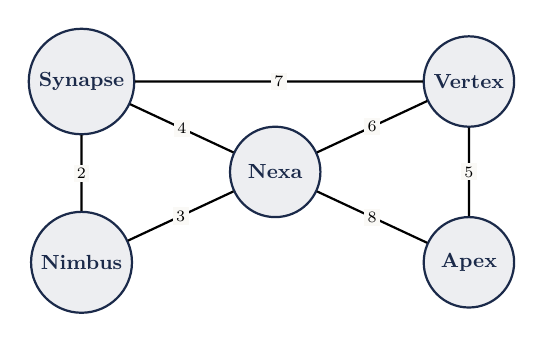
\begin{tikzpicture}[scale=0.82, every node/.style={transform shape},
  node distance=1cm,
  dc/.style={circle, draw=primary, thick, fill=primary!8, minimum size=1.4cm, font=\small\bfseries\color{primary}},
  edgelabel/.style={font=\scriptsize, fill=paper, inner sep=1.5pt}
]
  \node[dc] (nexa) at (0,0) {Nexa};
  \node[dc] (syn)  at (-3.0,1.4) {Synapse};
  \node[dc] (vtx)  at (3.0,1.4) {Vertex};
  \node[dc] (nim)  at (-3.0,-1.4) {Nimbus};
  \node[dc] (apx)  at (3.0,-1.4) {Apex};

  \draw[thick] (nexa) -- node[edgelabel]{4} (syn);
  \draw[thick] (nexa) -- node[edgelabel]{6} (vtx);
  \draw[thick] (nexa) -- node[edgelabel]{3} (nim);
  \draw[thick] (nexa) -- node[edgelabel]{8} (apx);
  \draw[thick] (syn)  -- node[edgelabel]{2} (nim);
  \draw[thick] (vtx)  -- node[edgelabel]{5} (apx);
  \draw[thick] (syn)  -- node[edgelabel]{7} (vtx);
\end{tikzpicture}
\end{center}
\vspace{0.5mm}

\question{10}{Model the network as a weighted graph. Write the adjacency matrix for the five data centers (order: Nexa, Synapse, Vertex, Nimbus, Apex), using $\infty$ for absent links.}
\solution{
\[
\begin{blockarray}{cccccc}
 & \text{Nexa} & \text{Syn} & \text{Vtx} & \text{Nim} & \text{Apx} \\
\begin{block}{c[ccccc]}
\text{Nexa} & 0 & 4 & 6 & 3 & 8 \\
\text{Syn}  & 4 & 0 & 7 & 2 & \infty \\
\text{Vtx}  & 6 & 7 & 0 & \infty & 5 \\
\text{Nim}  & 3 & 2 & \infty & 0 & \infty \\
\text{Apx}  & 8 & \infty & 5 & \infty & 0 \\
\end{block}
\end{blockarray}
\]
}
\answerlines{5}

\question{15}{Apply Dijkstra's algorithm starting from \textbf{Nimbus} to find the shortest-latency path to \textbf{Apex}. Show the running distance table after each vertex is finalized.}
\solution{
\begin{tabular}{@{}lccccc@{}}
\toprule
Step & Nexa & Synapse & Vertex & Nimbus & Apex \\
\midrule
Init & $\infty$ & $\infty$ & $\infty$ & 0 & $\infty$ \\
Finalize Nimbus (0) & 3 & 2 & $\infty$ & --- & $\infty$ \\
Finalize Synapse (2) & 3 & --- & 9 & --- & $\infty$ \\
Finalize Nexa (3) & --- & --- & 9 & --- & 11 \\
Finalize Vertex (9) & --- & --- & --- & --- & 11 \\
\bottomrule
\end{tabular}\\{}
Shortest path: \textbf{Nimbus $\to$ Synapse $\to$ Nexa $\to$ Apex} with total latency \textbf{11\,ms} (via Nexa is cheaper than the direct Vertex--Apex leg, $9+5=14$).}
\answerlines{6}

\question{15}{The operations team is deciding between an adjacency matrix and an adjacency list representation for this network as it scales to $V = 500$ data centers with $E \approx 1500$ links. Justify, with complexity analysis, which representation --- and which shortest-path algorithm variant --- they should choose.}
\solution{An adjacency matrix costs $O(V^2)$ space and makes Dijkstra's edge-relaxation step $O(V^2)$ overall, which is wasteful for a \emph{sparse} graph ($E \ll V^2$; here $1500 \ll 500^2 = 250{,}000$). An adjacency list costs $O(V+E)$ space, and Dijkstra with a binary min-heap runs in $O((V+E)\log V)$, which for these parameters is dramatically faster than $O(V^2)$. \textbf{Recommendation:} adjacency list with a heap-based (priority-queue) Dijkstra implementation.}
\answerlines{5}

% =========================================================
\ifshowsolutions
\examsection{Answer Key}{Quick Reference}
\begin{center}
\renewcommand{\arraystretch}{1.1}
\begin{tabular}{@{}c c c c@{}}
\toprule
\rowcolor{primary!10}
\textbf{Q} & \textbf{Answer} & \textbf{Q} & \textbf{Answer} \\
\midrule
I.1 & C & III.1 & Proof (see above) \\
I.2 & B & III.2 & $O(n)$ pseudocode \\
I.3 & B & IV.1 & Adjacency matrix (see above) \\
I.4 & D & IV.2 & Nimbus--Synapse--Nexa--Apex, 11\,ms \\
I.5 & B & IV.3 & Adjacency list + heap Dijkstra \\
II.1--II.4 & See worked solutions & & \\
\bottomrule
\end{tabular}
\end{center}
\fi

\vspace{3mm}
\begin{center}
\small\color{slate}\textit{--- End of examination. Please verify you have answered all four parts before submitting. ---}
\end{center}

\end{document}
